% =====================================================================
% Data preparation pipeline — paper section + figure (drop-in).
% Self-contained: compiles on its own, or paste Section + figure(s)
% into data_and_scenarios_methodology.tex (it complements Section 5 there,
% which lists the individual build scripts; this is the readable overview).
% Figure assets: fig_data_preparation_pipeline.pdf (rendered, vector) and
% an equivalent native-TikZ figure below. Use whichever you prefer.
% =====================================================================
\documentclass[11pt,a4paper]{article}
\usepackage[utf8]{inputenc}\usepackage[T1]{fontenc}\usepackage{lmodern}
\usepackage[margin=2.3cm]{geometry}\usepackage{amsmath,amssymb}
\usepackage{booktabs}\usepackage{xcolor}\usepackage{newunicodechar}
\usepackage{graphicx}\usepackage{tikz}\usetikzlibrary{arrows.meta,positioning,calc,fit}
\usepackage[hidelinks]{hyperref}
\setlength{\parskip}{0.5em}\setlength{\parindent}{0pt}
\definecolor{c1}{HTML}{2A78D6}\definecolor{c2}{HTML}{E8693A}\definecolor{c3}{HTML}{1BA784}
\definecolor{c4}{HTML}{1B3A6B}\definecolor{c5}{HTML}{D6537F}\definecolor{c6}{HTML}{0E8A16}
\newunicodechar{×}{\ensuremath{\times}}\newunicodechar{→}{\ensuremath{\rightarrow}}
\newunicodechar{−}{\ensuremath{-}}\newunicodechar{↔}{\ensuremath{\leftrightarrow}}
\newunicodechar{·}{\ensuremath{\cdot}}\newunicodechar{₂}{\ensuremath{_2}}
\begin{document}

\section*{Data preparation: from open-source data to model inputs}

The 2025 baseline is assembled entirely from open and audited data and then combined with the six Ariadne transition pathways. Preparation runs as three parallel tracks --- observed aviation data, observed maritime data, and the Ariadne scenario data --- each passing through the same five stages: collect \textbf{open-source sources}, \textbf{filter} to the German study fleet, \textbf{map/match} identities across datasets, \textbf{derive} per-asset activity and energy from raw records, and \textbf{calibrate} the technology catalog. The three tracks converge on the 24 case-input folders (three sectors $\times$ eight decision cases) that drive the NATM agent-based investment model. Figure~\ref{fig:dataprep} summarises the flow; the individual build scripts are listed in the construction section. Each stage is stated below together with \emph{what it determines} in the model.

\subsection*{Aviation track}

\textbf{Sources.} A global fleet export (Planespotters, 49{,}391 aircraft rows with type, operator, country, build/delivery dates, engines, seats, haul class and range); the public fleet pages of 18 German operators (tail registrations); the OpenSky Network aircraft database (registration~$\rightarrow$ ICAO24 transponder address); the OpenSky REST \texttt{/flights/all} service (observed global flights); the OpenAP aircraft-performance model (TU~Delft) for physics-based fuel and emissions; the ICAO/EASA Emissions Databank for certified non-CO₂ factors; Eurostat for an independent fleet-count benchmark; and a compiled aircraft-price workbook for CAPEX anchors.

\textbf{Filter.} The export is restricted to German commercial passenger and freight operators (49k~$\rightarrow$ 787 aircraft), yielding the realised baseline of 474 passenger aircraft and 74 freighters; the count is validated against the Eurostat benchmark (480 passenger, 119 cargo for Germany).

\textbf{Map / match.} Because the export carries attributes but no registration, each pasted registration is matched to a fleet record on operator, type family and delivery year/month (falling back to year only where a lease or transfer moved the delivery date), and bucketed as matched, ambiguous, no-candidate or too-new. Registrations are then resolved to ICAO24 addresses through the OpenSky database (484 of~600) and the SkyLink registry API (a further~85). Aircraft types not supported by OpenAP are mapped to the nearest supported type through a logged fallback table.

\textbf{Derive.} Global flight records are filtered to the fleet's ICAO24 set (496{,}778 matched flights; Unix-second timestamps converted to UTC), each flight's fuel, energy and pollutant emissions are modelled in OpenAP (450{,}129 flights), and the results are aggregated into per-aircraft activity profiles: annual departures, mean stage length, annual distance, a distance-weighted domestic/international split computed per registration, and a baseline annual energy demand.

\textbf{Calibrate.} The technology catalog is anchored to real values: CAPEX from the price workbook (USD~$\rightarrow$ EUR at quote-year average rates); non-CO₂ factors from the EDB; the CO₂ factor corrected to 0.2636~kg\,CO₂/kWh on an EU~ETS, fuel-LHV basis; energy intensity (km/kWh) replaced by the empirical per-aircraft value; and evidence-based lifetimes.

\textbf{Determines:} the 2025 passenger and cargo fleet stock, each asset's utilisation and energy demand, the emission factors charged in operation, and the per-segment menu of renewal options.

\subsection*{Maritime track}

\textbf{Sources.} Audited EU~MRV CO₂-monitoring reports (2021--2025) for per-vessel fuel use and energy intensity; Global Fishing Watch (GFW) 2024 port-visit events; the BSH register for validation; gross-tonnage and techno-economic cost tables; IMO emission factors; and the \texttt{searoute} library for leg distances.

\textbf{Filter.} Vessels are restricted to German entities and split by a gross-tonnage rule (40{,}000~GT separating regional from deep-sea), giving 131 German-flag cargo vessels, validated against the BSH register.

\textbf{Map / match.} Vessel identity is rebuilt around the IMO number, joining the MRV \texttt{Name}/\texttt{Company} fields, GFW name and flag, and manual lookups; MRV energy intensity is merged per vessel from the most recent reporting year carrying a value.

\textbf{Derive.} Consecutive GFW port visits are chained into voyage legs; \texttt{searoute} distances (cross-checked against great-circle) are computed over 6{,}213 legs; leg fuel is MRV kg per nautical mile times distance; activity profiles apply nm~$\rightarrow$ km ($\times$1.852) and MWh/nm~$\rightarrow$ kWh conversions, with the main hub taken from AIS port time where available.

\textbf{Calibrate.} The option menu is expanded from 6 to 20 technologies following the vessel taxonomy; CAPEX is ID-joined from the cost tables (with conversion/retrofit premia); efficiency and the CO₂ factor are calibrated to MRV, non-CO₂ factors taken from IMO, and lifetimes set from the vessel evidence.

\textbf{Determines:} the 2025 vessel stock and identity, each vessel's activity and energy, and the maritime technology catalog.

\subsection*{Ariadne pathway track}

\textbf{Sources.} The six Ariadne transition pathways supply energy-system price forecasts, transport-demand indices, and the belief-set probabilities used by the ambiguity-aware cases.

\textbf{Map / derive.} Forecast price columns are mapped to the model's per-carrier price variables (kerosene, SAF, e-kerosene, hydrogen, electricity, marine diesel, biofuel, LNG, methanol, ammonia), one value per pathway and milestone year (2030/35/40/45), held flat within each five-year block. Electricity prices are activity-weighted across the 672 quarter-hours of a representative week by observed activity shares (OpenSky departure times for aviation, GFW port-visit times for maritime):
\[
\bar{p}_{c,p,y}=\frac{\sum_k w_k\,p_{c,p,y}(\tau_k)}{\sum_k w_k}.
\]
Demand trajectories are the 2025 activity anchor times the pathway's demand index.

\textbf{Determines:} the scenario prices, demand trajectories and belief probabilities that distinguish the eight cases; the pathways reach the model \emph{only} through these inputs, never through the observed baseline.

\subsection*{Integration}

The three tracks populate 24 case-input folders, each holding a fleet-stock-plus-activity file, a technology catalog, a scenario file (prices and demand), and the belief-set probabilities. The NATM agent-based model then makes an annual NPV (risk-neutral) or robust (ambiguity-aware) technology choice over 2025--2050, producing technology per asset-year, energy and CO₂ by carrier, and electricity-equivalent demand.

\subsection*{Constructing the observed fleet dataset}

The observed baseline is computed per asset from raw movement records, not assumed. Figure~\ref{fig:fleetdata} shows the two per-asset pipelines.

\textbf{Aviation.} For each matched flight, the route distance is the great-circle distance between the departure and arrival airport coordinates (Earth radius $R = 6371$~km). A synthetic mission profile is generated in OpenAP --- climb, cruise and descent, with cruise altitude and true airspeed set by distance and the trajectory discretised into time steps $\Delta t$. Fuel is obtained by integrating the OpenAP fuel-flow $\dot f$ along the profile while the aircraft mass is reduced each step,
\[
m_{\text{fuel}} \;=\; \sum_k \dot f(\tau_k)\,\Delta t_k ,
\]
then converted to energy and CO₂ as $E[\text{MWh}] = m_{\text{fuel}}\cdot \text{LHV}/3600$ (Jet~A-1 LHV $\approx 43$~MJ/kg) and $m_{\text{CO}_2} = 3.16\,m_{\text{fuel}}$, with non-CO₂ species from the OpenAP emission model. Summing each aircraft's flights gives its annual departures, annual distance, mean stage length, distance-weighted domestic/international split and baseline energy demand.

\textbf{Maritime.} EU~MRV filings report each vessel's annual fuel and CO₂ and a fuel intensity $i$ in kg per nautical mile. Consecutive GFW port visits are chained into voyage legs; the per-leg \texttt{searoute} sea distance (cross-checked against great-circle) is summed to the annual distance, and annual fuel is the reported MRV total, or $\sum_\ell i\, d_\ell$ where not reported. The energy intensity is $i\cdot\text{LHV}/3600$ (MWh per nautical mile), and distances convert with $1$~n\,mile $= 1.852$~km. Aggregation per vessel yields voyages, annual distance, annual fuel and energy, and the main hub from AIS port time.

\begin{figure}[htbp]\centering
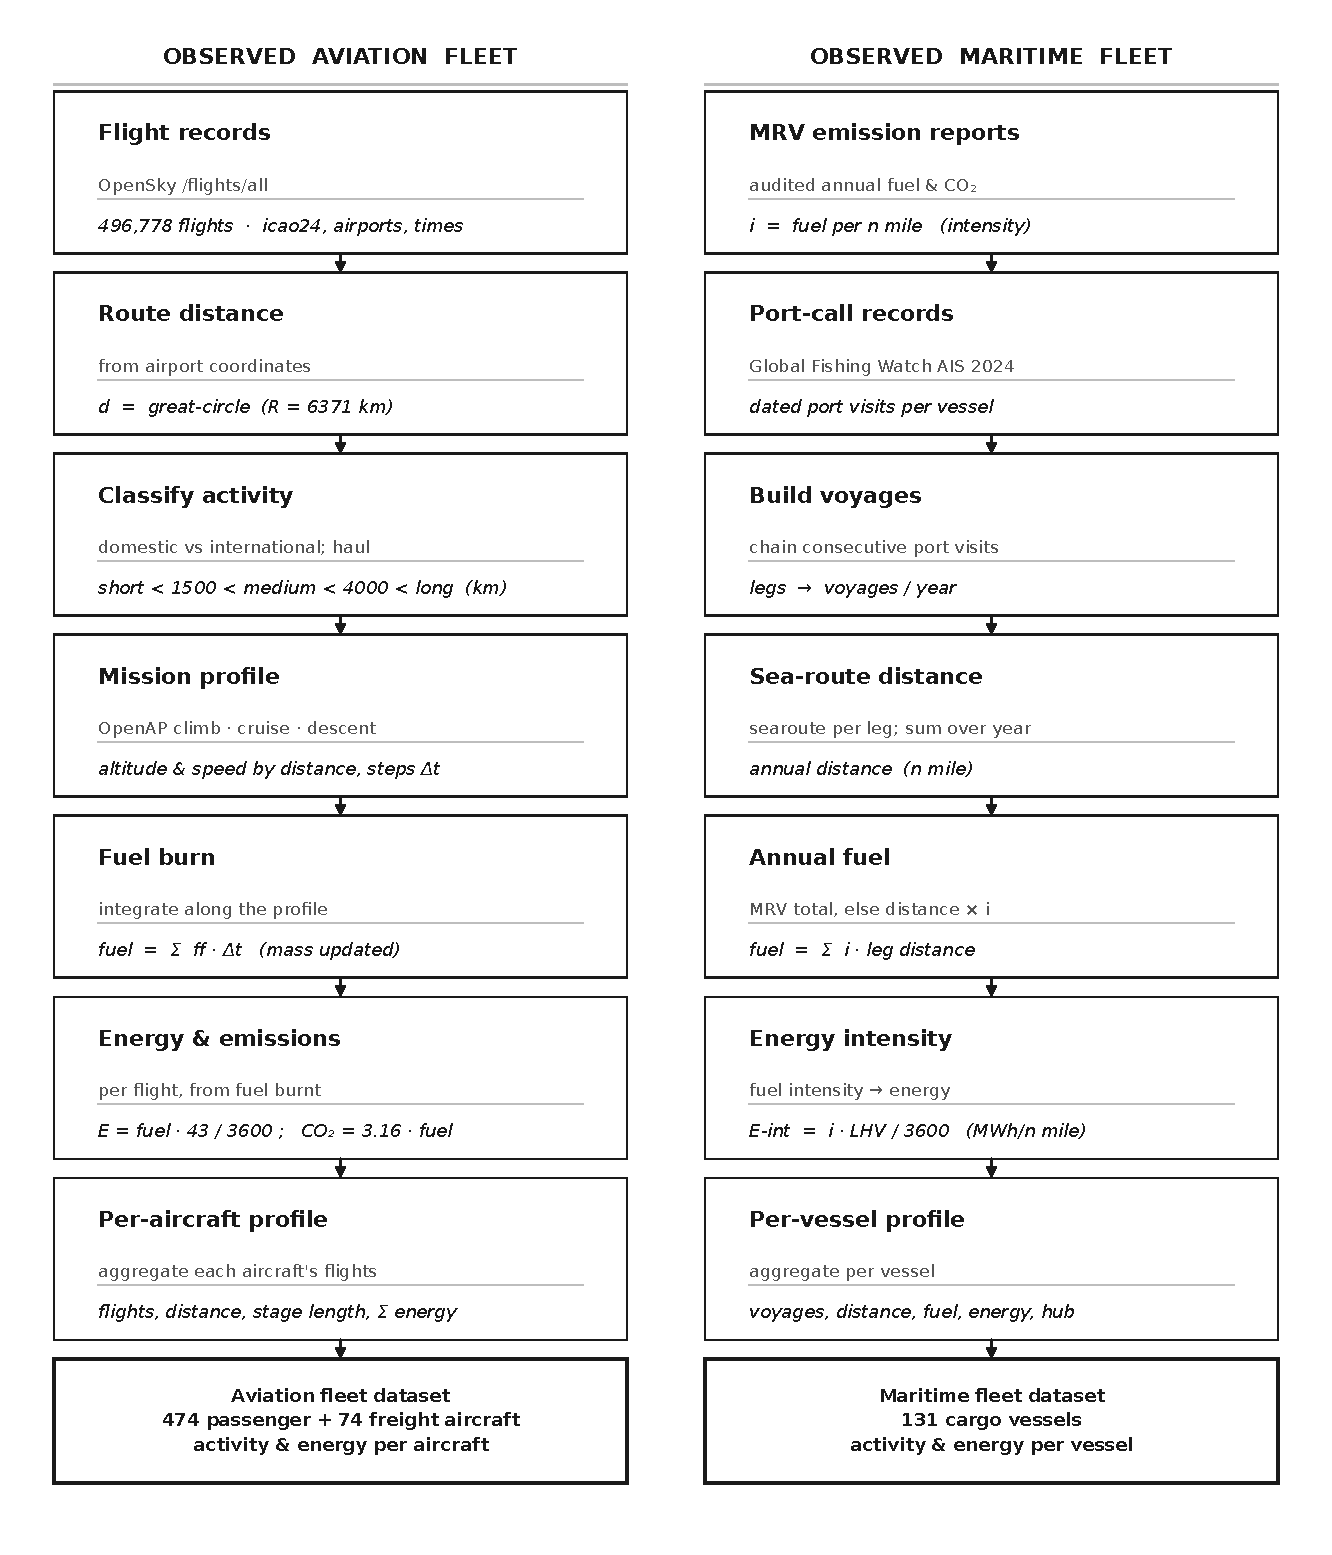
\includegraphics[width=\linewidth]{fig_fleet_dataset_construction.pdf}
\caption{Construction of the observed per-asset fleet datasets. Each column is a pipeline from raw open records to a calibrated per-asset baseline; the rule inside every box separates the step's description from its calculation. Aviation fuel is integrated flight-by-flight in OpenAP; maritime fuel follows from audited EU~MRV intensities and AIS-derived voyage distances.}
\label{fig:fleetdata}
\end{figure}

% ---------------------------------------------------------------------
% OPTION A — rendered vector figure (overview flow; recommended).
% ---------------------------------------------------------------------
\begin{figure}[htbp]\centering
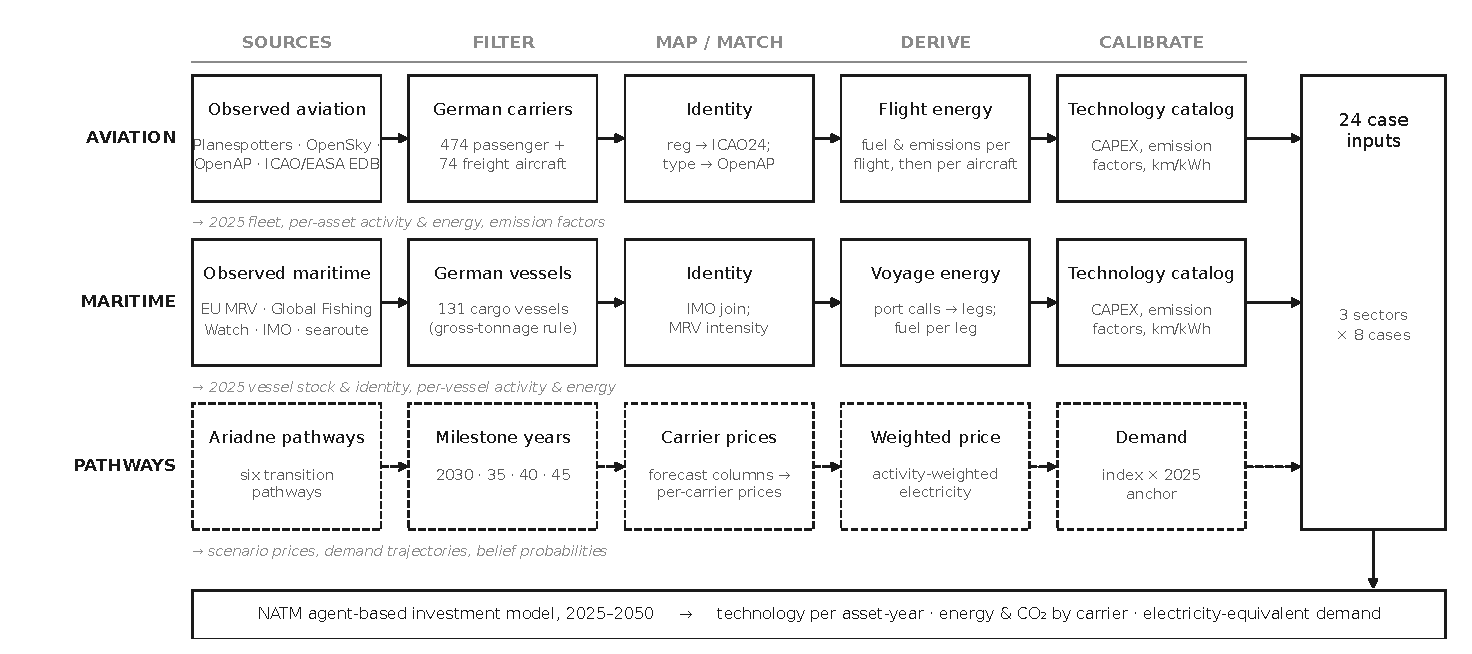
\includegraphics[width=\linewidth]{fig_data_preparation_pipeline.pdf}
\caption{Data preparation from open-source data to NATM model inputs. Each track passes through filter, map/match, derive and calibrate stages; the italic line below names what it determines. The two observed-data tracks (aviation, maritime) use solid outlines; the Ariadne-pathway track is dashed to mark it as scenario, not observed, data. All three converge on the 24 case inputs that drive the agent-based model.}
\label{fig:dataprep}
\end{figure}

% ---------------------------------------------------------------------
% OPTION B — native TikZ equivalent (same content; delete Option A if used).
% ---------------------------------------------------------------------
\begin{figure}[htbp]\centering
\footnotesize
% Monochrome journal style: hairline boxes, no fill, pathway row dashed.
\begin{tikzpicture}[font=\scriptsize, x=3.15cm, y=1cm, line width=0.5pt,
  stg/.style={draw=black, align=center, text width=2.75cm, inner sep=3pt, minimum height=2.3cm},
  pth/.style={stg, densely dashed},
  hd/.style={font=\footnotesize\bfseries, text=gray, align=center},
  sub/.style={text=gray}, rl/.style={font=\footnotesize\bfseries, anchor=east},
  arr/.style={-{Stealth[length=2mm]}, black},
  arrp/.style={-{Stealth[length=2mm]}, black, densely dashed},
  det/.style={font=\scriptsize\itshape, text=gray, anchor=north west}]
% headers
\node[hd] at (0,2.0){Sources}; \node[hd] at (1,2.0){Filter}; \node[hd] at (2,2.0){Map / match};
\node[hd] at (3,2.0){Derive}; \node[hd] at (4,2.0){Calibrate}; \node[hd] at (5.25,2.0){Inputs};
% aviation
\node[rl] at (-0.55,0){AVIATION};
\node[stg] (a0) at (0,0){Observed aviation\\[2pt]{\sub Planespotters · OpenSky · OpenAP · ICAO/EASA EDB}};
\node[stg] (a1) at (1,0){German carriers\\[2pt]{\sub 474 pax + 74 freight}};
\node[stg] (a2) at (2,0){Identity\\[2pt]{\sub reg→ICAO24; type→OpenAP}};
\node[stg] (a3) at (3,0){Flight energy\\[2pt]{\sub fuel \& emissions per flight}};
\node[stg] (a4) at (4,0){Technology catalog\\[2pt]{\sub CAPEX, factors, km/kWh}};
\node[det] at (-0.55,-1.35){→ 2025 fleet, per-asset activity \& energy, emission factors};
% maritime
\node[rl] at (-0.55,-3.3){MARITIME};
\node[stg] (m0) at (0,-3.3){Observed maritime\\[2pt]{\sub EU MRV · GFW · IMO · searoute}};
\node[stg] (m1) at (1,-3.3){German vessels\\[2pt]{\sub 131 cargo vessels}};
\node[stg] (m2) at (2,-3.3){Identity\\[2pt]{\sub IMO join; MRV intensity}};
\node[stg] (m3) at (3,-3.3){Voyage energy\\[2pt]{\sub port calls→legs; fuel/leg}};
\node[stg] (m4) at (4,-3.3){Technology catalog\\[2pt]{\sub CAPEX, factors, km/kWh}};
\node[det] at (-0.55,-4.65){→ 2025 vessel stock \& identity, per-vessel activity \& energy};
% pathways (dashed)
\node[rl] at (-0.55,-6.6){PATHWAYS};
\node[pth] (p0) at (0,-6.6){Ariadne pathways\\[2pt]{\sub six transition pathways}};
\node[pth] (p1) at (1,-6.6){Milestone years\\[2pt]{\sub 2030 · 35 · 40 · 45}};
\node[pth] (p2) at (2,-6.6){Carrier prices\\[2pt]{\sub forecast cols→carriers}};
\node[pth] (p3) at (3,-6.6){Weighted price\\[2pt]{\sub activity-weighted elec.}};
\node[pth] (p4) at (4,-6.6){Demand\\[2pt]{\sub index × 2025 anchor}};
\node[det] at (-0.55,-7.95){→ scenario prices, demand trajectories, belief probabilities};
% case-inputs panel
\node[stg, text width=1.9cm, minimum height=9.2cm] (ci) at (5.25,-3.3)
  {24 case inputs\\[3pt]{\sub 3 sectors × 8 cases}};
% row arrows
\foreach \i in {0,1,2,3}{\draw[arr] (a\i.east)--(a\the\numexpr\i+1\relax.west);}
\foreach \i in {0,1,2,3}{\draw[arr] (m\i.east)--(m\the\numexpr\i+1\relax.west);}
\foreach \i in {0,1,2,3}{\draw[arrp] (p\i.east)--(p\the\numexpr\i+1\relax.west);}
% convergence
\draw[arr]  (a4.east) -- (a4.east -| ci.west);
\draw[arr]  (m4.east) -- (ci.west);
\draw[arrp] (p4.east) -- (p4.east -| ci.west);
% downstream model
\node[stg, text width=12.2cm, minimum height=0.9cm, anchor=north west] (nm) at (0,-9.7)
  {NATM agent-based investment model, 2025–2050 \quad→\quad technology per asset-year · energy \& CO₂ by carrier · electricity-equivalent demand};
\draw[arr] (ci.south) -- (ci.south |- nm.north);
\end{tikzpicture}
\caption{Native-TikZ equivalent of the data-preparation flow (same content and style as the rendered Figure~\ref{fig:dataprep}); use this or the \texttt{\textbackslash includegraphics} version above, not both.}
\end{figure}

\end{document}
